\documentclass[10pt, compress, handout]{beamer}

\usetheme{utopia}

\usepackage{booktabs}
\usepackage[scale=2]{ccicons}
\usepackage[outputdir=out]{minted}
\usepackage{natbib}

\usepgfplotslibrary{dateplot}

\usetikzlibrary{shapes,arrows,positioning,intersections}
\tikzstyle{block} = [rectangle, draw, fill=blue!20,
    text width=5em, text centered, rounded corners, minimum height=4em]
\tikzstyle{line} = [draw, -latex']


\usemintedstyle{trac}

\hypersetup{colorlinks=false}

\title{Control Theory in Biology}
\subtitle{}
\date{15.06.2022}
\author{Jonas Pleyer}
\institute{Freiburg Center for Data Analysis and Modeling (FDM)}

\begin{document}

\maketitle

\section{Introduction}
\label{sec:introduction}
\subsection{What is Machine Learning?}
\label{subsec:introduction-definition}
\begin{frame}{\insertsubsection}
    'A computer program is said to learn from experience $E$ with respect to some class of tasks $T$ and performance measure $P$ if its performance at tasks in $T$, as measured by $P$, improves with experience $E$'\\
    - Tom M. Mitchell~\cite{Mitchell1997}
\end{frame}
%
%
\subsection{History of Machine Learning}
\label{subsec:introduction-history}
\begin{frame}{\insertsubsection}
    \begin{itemize}[<+->]
        \item[1943] First publication of neural network~\cite{McCulloch1943}
        \item[1956] Dartmouth Summer Research Project (Birthplace of modern Machine Learning)
        \item[1965] Nilson Machine Learning for pattern classification~\cite{Nilsson1965}
        \item[1966] Following years: Many setbacks in Artificial Intelligence called 'AI-Winters'
        \item[1995] Support Vector Machines are first introduced
        \item[2002] Torch first release (open source library)
        \item[2006] Geoffrey Hinton coins 'Deep Learning'~\cite{Hinton2006}
        \item[>2006] Companies such as Netflix, Facebook, Microsoft, Google fund projects/prizes in and use machine learning/artificial intelligence
    \end{itemize}
\end{frame}
%
%
\subsection{Workflow}
\label{subsec:introduction-workflow}
\begin{frame}{\insertsubsection}
    Machine learning techniques follow a similar workflow.
    \begin{enumerate}[<+->]
        \item Define Problem (scope, feasability)
        \item Gather Data (assumptions, constraints)
        \item Pre-process Data (cleanup, drop)
        \item Analyze Data (define features, find correlations)
        \item Prepare Data (transform, normalize, drop)
        \item Evaluate Models (train/test, classify/regress)
        \item Tune Model (cross validation, fine tune parameters)
        \item Apply model to problems, learn more
    \end{enumerate}
\end{frame}
\section{Examples from Biology}
\label{sec:examples}
\subsection{Child Birth}
\label{subsec:examples-pregnancy}
\begin{frame}{\insertsubsection}
    \begin{figure}
        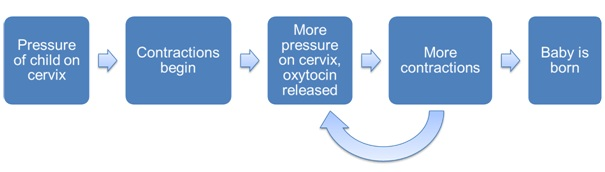
\includegraphics[width=\textwidth]{media/Childbirth.jpg}
        \caption{Childbirth~\cite{albert2022}}
    \end{figure}
    \begin{itemize}[<+->]
        \item More pressure 
        \item[ ] $\rightarrow$ More contractions
        \item This is a \emph{positive feedback loop}.
    \end{itemize}
\end{frame}
%
%
\subsection{Temperature Regulation}
\label{subsec:examples-temperature}
\begin{frame}{\insertsubsection}
    \begin{minipage}[t]{0.349\textwidth}
        \begin{itemize}[<+->]
            \item More Sweat
            \item[ ] $\rightarrow$ Less Temperature
            \item More ...
            \item[ ] $\rightarrow$ Less ...
            \item This is a \emph{negative feedback loop}.
        \end{itemize}
    \end{minipage}%
    \begin{minipage}[t]{0.649\textwidth}
        \begin{figure}
            \centering
            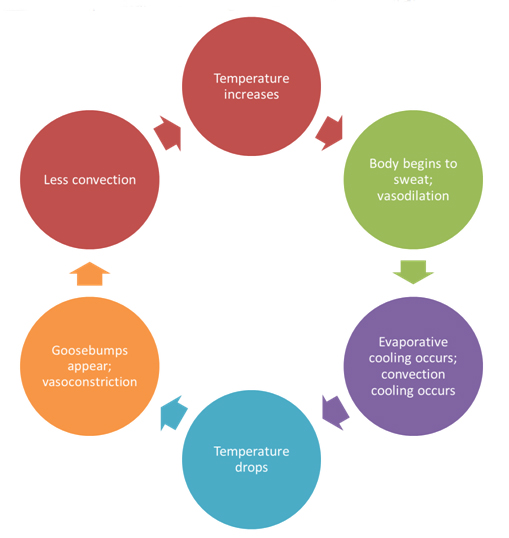
\includegraphics[width=\textwidth]{media/Temperature-Regulation.jpg}
            \caption{Temperature regulation~\cite{albert2022}}
        \end{figure}
    \end{minipage}%
\end{frame}
%
%
\subsection{More Examples}
\label{subsec:more-examples}
\begin{frame}{\insertsubsection}

    \begin{itemize}[<+->]
        \item Tight calcium regulation in humans
        \item Receptor Networks
        \item Synthetic Biology
        \item Optogenetics (What we also do)
        \item Financial Markets
        \item Social Relationships
        \item ...
    \end{itemize}
\end{frame}
%
%
\section{Concepts}
\label{sec:concepts}
\subsection{Closed and Open Loop}
\label{subsec:concepts-closed-open-loop}
\begin{frame}{\insertsubsection}
	We distinguish between two different controllers
	\begin{itemize}
		\item Open Loop Controller
		\item Closed Loop Controller
		\item[ ] $\rightarrow$ Closed loop control schemes are the biologically more interesting ones.
	\end{itemize}
\end{frame}
%
%
\begin{frame}{\insertsubsection}
\begin{figure}
	\begin{tikzpicture}
		% Draw nodes
		\node [block] (controller) {Controller};
		\coordinate [left of=controller, node distance=3cm] (init);
		\node [block, right of=controller, node distance=5cm] (system) {System};
		\coordinate [right of=system, node distance=3cm] (end);
		% Draw lines connecting (arrows)
		\path [line] (init) -- node [midway, above] {Input} (controller);
		\path [line] (controller) -- node [midway, above] {Control Signal} (system);
		\path [line] (system) -- node [midway, above] {Output} (end);
	\end{tikzpicture}
	\caption{Open Loop Control System}
\end{figure}
\end{frame}
%
%
\begin{frame}{\insertsubsection}
\begin{figure}
	\begin{tikzpicture}
		% Draw nodes
		\node [block] (controller) {Controller};
		\node [block, right=3cm of controller] (system) {System};
		\node [block, below right=0.5cm and 0.5cm of controller] (measurement) {Measurement};
		% Helper coordinates
		\coordinate [left=2cm of controller] (init);
		\coordinate [right=2cm of system] (end);
		\coordinate [right=1cm of system] (measurepoint);
		\coordinate [below right=0.5cm and 5cm of controller] (rightcorner);
		\coordinate [below of=controller] (leftcorner);
		% Draw lines connecting (arrows)
		\path [line] (init) -- node [midway, above] {Input} (controller);
		\path [line] (controller) -- node [midway, above] {Control Signal} (system);
		\path [line] (system) -- node [midway, above] {Output} (end);
		% \path [line] (measurepoint) -- (rightcorner) -- (measurement);
		%\draw (measurepoint) to (rightcorner) to (measurement) to (leftcorner) to (controller);
		\path [line] (measurepoint) |- (measurement);
		\path [line] (measurement) -| (controller);
	\end{tikzpicture}
	\caption{Closed Loop Control System with Measurement and Feedback}
\end{figure}
\end{frame}
%
%
\subsection{Controller Types}
\label{subsec:concepts-controller-types}
\begin{frame}{\insertsubsection}
	\begin{figure}
		\centering
		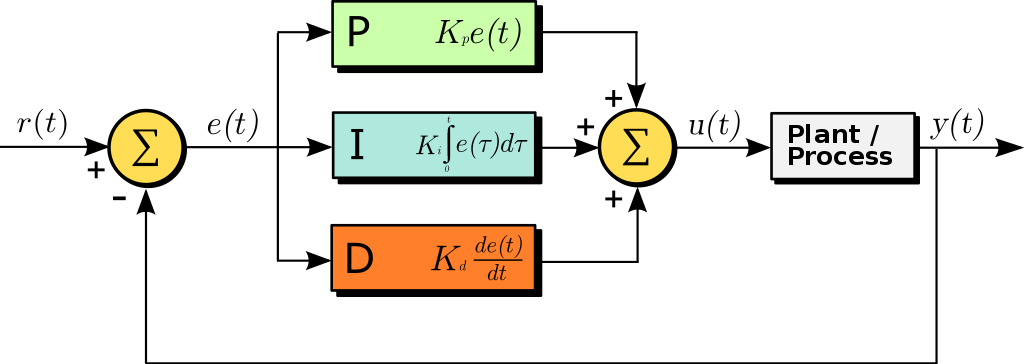
\includegraphics[width=\textwidth]{media/PID_en}
		\caption{Schematic Overview of a Controller~\cite{wikiPID2011}}
	\end{figure}
	Relevant values:\\
	$u(t)$ - Response of controller\\
	$e(t)$ - Difference of input signal and setpoint (target)
	\begin{equation}
		e(t) = r(t) - y(t)
	\end{equation}
\end{frame}
%
%
\subsubsection{Proportional (P) Controller}
\label{subsec:concepts-controller-types-p-controller}
\begin{frame}{\insertsubsubsection}
	$u(t)$ - Response of controller\\
	$e(t)$ - Difference of input signal and setpoint (target)\\\\
	We want to calculate response $u(t)$ from input $e(t)$.\\
	Use a proportional response
	\begin{equation}
		u(t) = K_P e(t)
	\end{equation}
\end{frame}
%
%
\subsubsection{Differential (D) Controller}
\label{subsec:concepts-controller-types-d-controller}
\begin{frame}{\insertsubsubsection}
	$u(t)$ - Response of controller\\
	$e(t)$ - Difference of input signal and setpoint (target)\\\\
	Differential response
	\begin{equation}
		u(t) = K_D \frac{\partial e}{\partial t}
	\end{equation}
	In discretized version
	\begin{equation}
		u(t_{i+1}) = K_D \frac{e(t_{i+1})- e(t_i)}{\Delta t}
	\end{equation}
\end{frame}
%
%
\subsubsection{Integral (I) Controller}
\label{subsec:concepts-controller-types}
\begin{frame}{\insertsubsubsection}
	$u(t)$ - Response of controller\\
	$e(t)$ - Difference of input signal and setpoint (target)\\\\
	Differential response
	\begin{equation}
		u(t) = K_I \int\limits^t_0 e(\tau)d\tau
	\end{equation}
	In discretized version
	\begin{equation}
		u(t_{n+1}) = K_I \sum\limits_{i=0}^n e(t_i)\Delta t
	\end{equation}
\end{frame}
%
%
\subsection{Combinations of Controller}
\label{subsec:concepts-combinations}
\begin{frame}{\insertsubsection}
	We can combine the previously introduced controllers.\\
	PD Controller
	\begin{equation}
		u(t) = K_P e(t) + K_D \frac{\partial e}{\partial t}
	\end{equation}
	PI Controller
	\begin{equation}
		u(t) = K_P e(t) + K_I \int\limits^t_0 e(\tau)d\tau
	\end{equation}
	PID Controller
	\begin{equation}
		u(t) = K_P e(t) + K_I \int\limits^t_0 e(\tau)d\tau + K_D \frac{\partial e}{\partial t}
	\end{equation}
	...
\end{frame}
%
%
\subsubsection{Controller Constants}
\label{subsec:concepts-controller-constant-discussion}
\begin{frame}{\insertsubsubsection}
	\begin{figure}
		\centering
		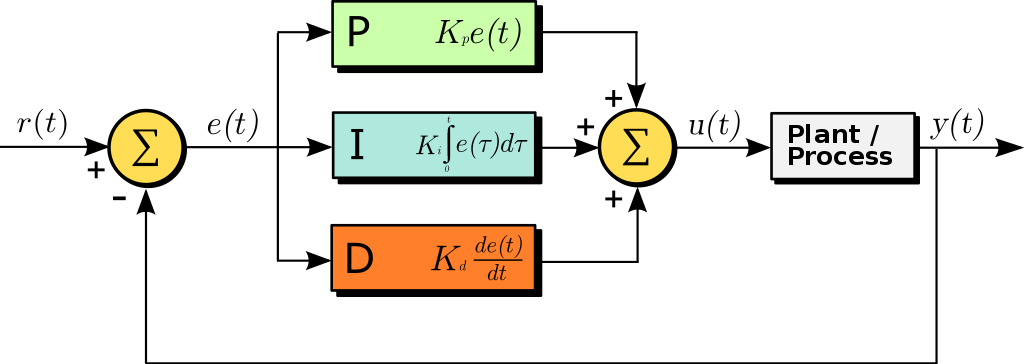
\includegraphics[width=\textwidth]{media/PID_en}
		\caption{Schematic Overview of a PID Controller~\cite{wikiPID2011}}
	\end{figure}
	\begin{align}
		e(t) &= r(t) - y(t)\\
		u(t) &= K_P e(t) + K_I \int\limits^t_0 e(\tau)d\tau + K_D \frac{\partial e}{\partial t}
	\end{align}
\end{frame}
%
%
\begin{frame}{\insertsubsubsection}
	What do the parameters $K_P, K_I, K_D$ do?
	\begin{equation}
		u(t) = K_P e(t) + K_I \int\limits^t_0 e(\tau)d\tau + K_D \frac{\partial e}{\partial t}
	\end{equation}
	Alternative representation
	\begin{equation}
		u(t) = K_P \left(e(t) + \frac{1}{T_I}\int\limits^t_0 e(\tau)d\tau + T_D\frac{\partial e}{\partial t}\right)
	\end{equation}
	What do $K_p,T_I,T_D$ do now?
\end{frame}
%
%
\begin{frame}{\insertsubsubsection}
	\begin{figure}
		\centering
		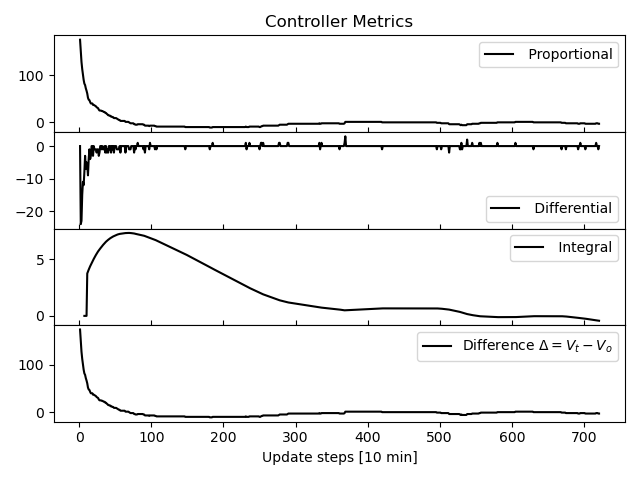
\includegraphics[width=0.8\textwidth]{media/UkrainianFlagControllerMetrics}
		\caption{Optimal Control for a given system.}
	\end{figure}
\end{frame}
%
%
\begin{frame}{\insertsubsubsection}
	\begin{figure}
		\centering
		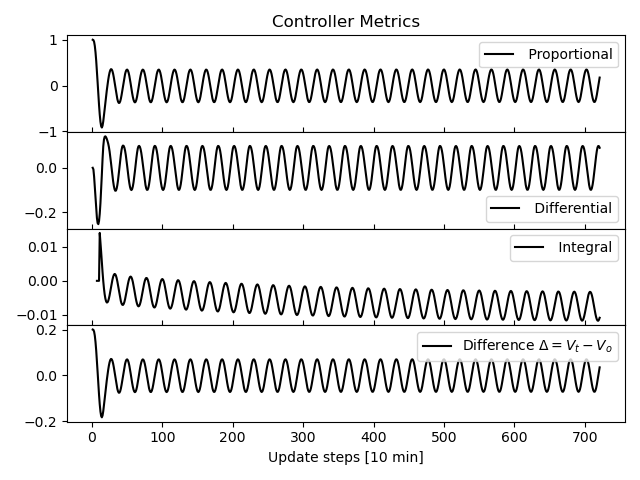
\includegraphics[width=0.8\textwidth]{media/TimeDelayOscillations}
		\caption{Oscillations can occur upon time-delays are.}
	\end{figure}
\end{frame}
%
%
\subsection{Optogenetic Control}
\label{subsec:concepts-optogenetic-control}
\begin{frame}{\insertsubsubsection}
	\begin{figure}
		\centering
		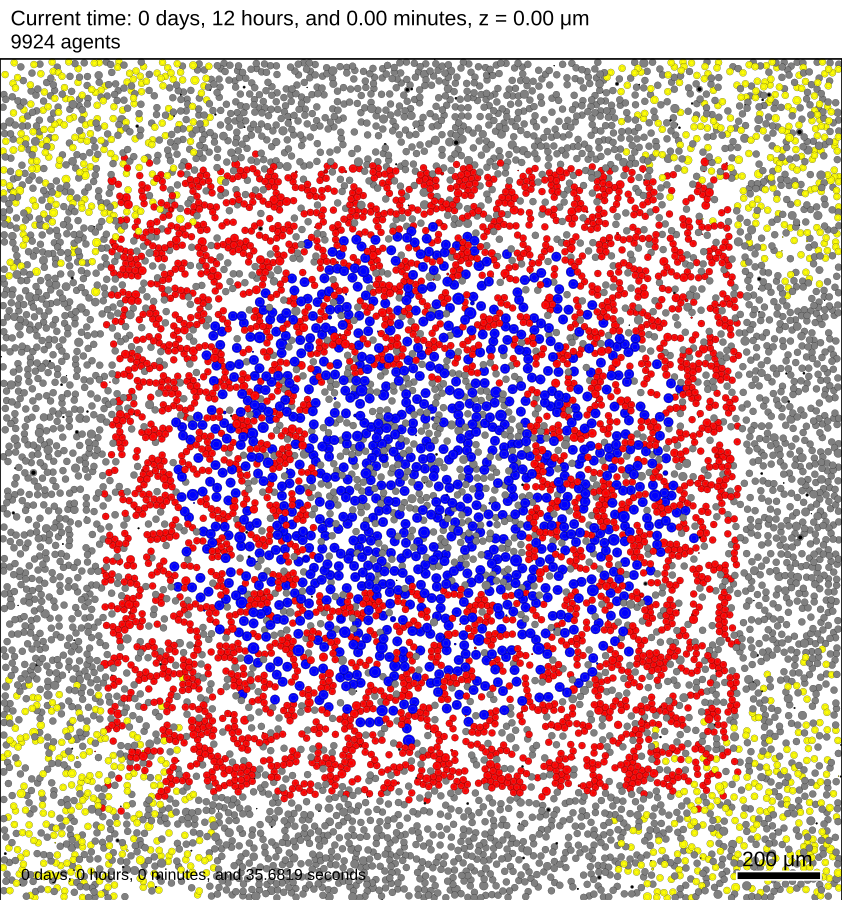
\includegraphics[width=0.6\textwidth]{media/SpatialDensityControl}
		\caption{Optogenetic controllers regulate cell densities in different spatial compartiments.}
	\end{figure}
\end{frame}
\section{Biology again}
\label{sec:biology-again}
\begin{frame}{\insertsubsection}
    
\end{frame}

% \begin{frame}[fragile]
%   \frametitle{Sections}
%   Sections group slides of the same topic
% 
%   \begin{minted}[fontsize=\small]{latex}
%     \section{Elements}
%   \end{minted}
% 
%   for which the \emph{mtheme} provides a nice progress indicator \ldots
% \end{frame}
% 
% \section{Elements}
% 
% \begin{frame}[fragile]
%   \frametitle{Typography}
%       \begin{minted}[fontsize=\small]{latex}
% The theme provides sensible defaults to \emph{emphasize}
% text, \alert{accent} parts or show \textbf{bold} results.
%       \end{minted}
% 
%   \begin{center}becomes\end{center}
% 
%   The theme provides sensible defaults to \emph{emphasize} text,
%   \alert{accent} parts or show \textbf{bold} results.
% \end{frame}
% \begin{frame}{Lists}
%   \begin{columns}[onlytextwidth]
%     \column{0.5\textwidth}
%       Items
%       \begin{itemize}
%         \item Milk \item Eggs \item Potatos
%       \end{itemize}
% 
%     \column{0.5\textwidth}
%       Enumerations
%       \begin{enumerate}
%         \item First, \item Second and \item Last.
%       \end{enumerate}
%   \end{columns}
% \end{frame}
% \begin{frame}{Descriptions}
%   \begin{description}
%     \item[PowerPoint] Meeh.
%     \item[Beamer] Yeeeha.
%   \end{description}
% \end{frame}
% \begin{frame}{Animation}
%   \begin{itemize}[<+- | alert@+>]
%     \item \alert<4>{This is\only<4>{ really} important}
%     \item Now this
%     \item And now this
%   \end{itemize}
% \end{frame}
% \begin{frame}{Tables}
%   \begin{table}
%     \caption{Largest cities in the world (source: Wikipedia)}
%     \begin{tabular}{lr}
%       \toprule
%       City & Population\\
%       \midrule
%       Mexico City & 20,116,842\\
%       Shanghai & 19,210,000\\
%       Peking & 15,796,450\\
%       Istanbul & 14,160,467\\
%       \bottomrule
%     \end{tabular}
%   \end{table}
% \end{frame}
% \begin{frame}{Blocks}
% 
%   \begin{block}{This is a block title}
%     This is soothing.
%   \end{block}
% 
% \end{frame}
% \begin{frame}{Math}
%   \begin{equation*}
%     e = \lim_{n\to \infty} \left(1 + \frac{1}{n}\right)^n
%   \end{equation*}
% \end{frame}
% \begin{frame}{Line plots}
%   \begin{figure}
%     \begin{tikzpicture}
%       \begin{axis}[
%         mlineplot,
%         width=0.9\textwidth,
%         height=6cm,
%       ]
% 
%         \addplot {sin(deg(x))};
%         \addplot+[samples=100] {sin(deg(2*x))};
% 
%       \end{axis}
%     \end{tikzpicture}
%   \end{figure}
% \end{frame}
% \begin{frame}{Bar charts}
%   \begin{figure}
%     \begin{tikzpicture}
%       \begin{axis}[
%         mbarplot,
%         xlabel={Foo},
%         ylabel={Bar},
%         width=0.9\textwidth,
%         height=6cm,
%       ]
% 
%       \addplot plot coordinates {(1, 20) (2, 25) (3, 22.4) (4, 12.4)};
%       \addplot plot coordinates {(1, 18) (2, 24) (3, 23.5) (4, 13.2)};
%       \addplot plot coordinates {(1, 10) (2, 19) (3, 25) (4, 15.2)};
% 
%       \legend{lorem, ipsum, dolor}
% 
%       \end{axis}
%     \end{tikzpicture}
%   \end{figure}
% \end{frame}
% \begin{frame}{Quotes}
%   \begin{quote}
%     Veni, Vidi, Vici
%   \end{quote}
% \end{frame}
% 
% 
% \section{Conclusion}
% 
% \begin{frame}{Summary}
% 
%   Get the source of this theme and the demo presentation from
% 
%   \begin{center}\url{github.com/matze/mtheme}\end{center}
% 
%   The theme \emph{itself} is licensed under a
%   \href{http://creativecommons.org/licenses/by-sa/4.0/}{Creative Commons
%   Attribution-ShareAlike 4.0 International License}.
% 
%   \begin{center}\ccbysa\end{center}
% 
% \end{frame}
% 
\plain{Questions?}

\begin{frame}{Literature}[allowframebreaks]
    \bibliographystyle{alpha}
    \bibliography{ControlTheory}
\end{frame}
% 
%
\end{document}
